\documentclass[conference, 11pt]{IEEEtran}
\IEEEoverridecommandlockouts
% The preceding line is only needed to identify funding in the first footnote. If that is unneeded, please comment it out.
\usepackage{cite}
\usepackage{amsmath,amssymb,amsfonts}
\usepackage{algorithmic}
\usepackage{graphicx}
\usepackage{textcomp}
\usepackage{xcolor}
\usepackage{listings}

\def\BibTeX{{\rm B\kern-.05em{\sc i\kern-.025em b}\kern-.08em
    T\kern-.1667em\lower.7ex\hbox{E}\kern-.125emX}}
\begin{document}
\makeatletter % changes the catcode of @ to 11
\newcommand{\linebreakand}{%
  \end{@IEEEauthorhalign}
  \hfill\mbox{}\par
  \mbox{}\hfill\begin{@IEEEauthorhalign}
}
\makeatother % changes the catcode of @ back to 12


\title{Multi-threaded Chess AI\\
}

\author{\IEEEauthorblockN{Jonathan Cirillo}
\IEEEauthorblockA{\textit{Undergrad, Dept. Computer Science} \\
\textit{University of Central Florida}\\
Orlando, FL, USA \\
Cirillojon@knights.Ucf.edu}
\and
\IEEEauthorblockN{Jesse Johnson}
\IEEEauthorblockA{\textit{Undergrad, Dept. Computer Science} \\
\textit{University of Central Florida}\\
Orlando, FL, USA \\
j-jesse23@knights.ucf.edu}
\and
\IEEEauthorblockN{Lester Miller}
\IEEEauthorblockA{\textit{Undergrad, Dept. Computer Science} \\
\textit{University of Central Florida}\\
Orlando, FL, USA \\
lmiller44@knights.ucf.edu}
\and

\linebreakand

\IEEEauthorblockN{Marco Peric}
\IEEEauthorblockA{\textit{Undergrad, Dept. Computer Science} \\
\textit{University of Central Florida}\\
Orlando, FL, USA \\
mperic@knights.ucf.edu}
\and
\IEEEauthorblockN{Jonathan Velez}
\IEEEauthorblockA{\textit{Undergrad, Dept. Computer Science} \\
\textit{University of Central Florida}\\
Orlando, FL, USA \\
johnvelez01@knights.ucf.edu}
\and
\IEEEauthorblockN{}
\IEEEauthorblockA{\textit{} \\
\\
 \\
}
}

\maketitle

\begin{abstract}
For complex problems whose solutions tend to be time-consuming, one of the ways to improve runtime is through parallelization. Even for artificial intelligence (AI) algorithms that play complex games like chess, we can break down the processing time by parallelizing its main algorithm. This paper will be used to explore this potential in performance. We will use an algorithm that is commonly used in chess AIs called Alpha-Beta-Pruning. Alpha-Beta-Pruning is an optimization of the Minimax algorithm, which is used to find the best move in a 2-player game. By itself, the Alpha Beta algorithm increases the processing speed of the searching algorithm but we plan to improve its performance using parallelization. Using java, we successfully implemented three parallelizations of the Alpha Beta pruning algorithm, each using different parallelization methods. We then compare the performance of these parallelized versions to the sequential version, to determine if there was any improvement, and evaluate which technique was most effective. 
\end{abstract}

\begin{IEEEkeywords}
Alpha Beta pruning, Minimax, Parallel algorithms
\end{IEEEkeywords}

\section{Introduction}
Since its inception, chess has long been considered a challenging and complex game that requires players to memorize opening theory and predict their opponent's next moves. With the advancement in technology and the potential to incorporate Artificial Intelligence (AI) to play chess, there has been a significant improvement in chess AI. So much so that AI has long surpassed human capabilities when the IBM computer Deep Blue beat the chess grandmaster in 1997[1]. There are now plenty of algorithms that can beat humans in a game of chess, but we find that the same limitations that affect chess players also affect these algorithms: the number of moves that a player can look ahead is limited by resources and time.\vspace{10pt}

For simple games such as tic-tac-toe or checkers, an algorithm could determine the winning moves after a player's first or second move. But what makes chess such a complex game is the almost limitless amount of moves that a player can take. After just 3 moves from each player the pieces can have over nine million possible variations [2]. To address this challenge we attempt to parallelize a well-known chess search algorithm called Alpha Beta pruning using 3 different parallelization techniques. We will then demonstrate their effectiveness by measuring and comparing these implementation’s performance with the sequential Alpha Beta pruning.

\subsection{Minimax}

\begin{figure}[htbp]
\centerline{\includegraphics[scale=0.5]{ImageMinimax.png}}
\caption{Example of a Minimax algorithm.}
\label{fig}
\end{figure}

\subsection{Alpha Beta Pruning}

\begin{figure}[htbp]
\centerline{\includegraphics[scale=0.48]{ImageAlphaBetaPruning.png}}
\caption{Example of Alpha Beta pruning of the Minimax algorithm}
\label{fig}
\end{figure}

The minimax search tree is an algorithm that filters for the best move. At each level of depth, the node takes the alternative between the min and max value of their child nodes. With respect to chess, each depth represents the alternating moves between players and the values represent the state of the board after a move is made. This guarantees that after doing the search, the best move can be decided given a certain depth. 

Alpha-beta pruning: The algorithm begins by evaluating the root node of the tree, which represents the current state of the chess game. From this root node, the algorithm will explore all possible moves that can be made by the current chess position. The alpha and beta values to keep track of the best scores found so far for maximizing and minimizing each play. Initially, alpha is set to negative infinity, which means that any position score greater than negative infinity will become the new alpha value. Beta is set to positive infinity, which means that any position score less than positive infinity will become the new beta value.

When the algorithm evaluates each child node, it updates the alpha and beta values based on the scores found so far. During the search, alpha becomes greater than or equal to beta, then the algorithm can prune the current subtree. After all, it knows that any further exploration of this subtree will not contribute to the final result, since the subtree contains moves that are not optimal. When A child node is a maximizing node, then the algorithm updates the alpha value with the maximum score found so far. This means that a move will always choose the results in a score greater than or equal to the current alpha value. At the same time, a child node is given a minimizing node, then the algorithm updates the beta value with the minimum score. In other words, the algorithm aiming to minimize the score will consistently select a move that generates a score that is either equivalent to or lower than the present beta value.

\section{Alpha Beta In Chess}
The purpose of this study was to enhance the performance of the Alpha-Beta algorithm, utilizing parallelism, to more efficiently calculate a move for an AI in a chess game.
A high level overview of how the Alpha-Beta algorithm operates in the context of a chess game:
\begin{itemize}
  \item Assess each potential move from the current board position
  \item Identifies the optimal move for the current player
  \item The algorithm maintains alpha and beta values, representing the best scores discovered so far for maximizing and minimizing each play
  \item As the algorithm evaluates each child node, it updates the alpha and beta values based on the scores found up to that point
  \item Prunes the current subtree when alpha is greater than or equal to beta
\end{itemize}

Our team built off of an existing Java chess engine that features an AI implemented with a sequential Alpha-Beta algorithm, and used it as our base for parallelization.
This sequential code incorporates a board evaluator that assesses positions based on various criteria and search depth. The code also sorts moves according to various criteria, such as threat level and attack status. This sorting is referred to as “Move Ordering.” Move Ordering is performed to prioritize moves that have a higher chance of producing a positive result. By sorting the moves, it lets the algorithm explore these branches first, leading to earlier pruning, and more potential performance improvement. The Alpha-Beta search is performed in the ‘execute’ method. It takes in a Board object and returns the best move for the current player on the given board, as well as the execution time. The max and min helper methods are used to implement the core steps of the Alpha-Beta algorithm.

\begin{figure}[htbp]
\centerline{\includegraphics[scale=0.33]{alphaBetaChess.jpg}}
\caption{Alpha-Beta for Chess Positions}
\label{fig}
\end{figure}

\section{Implementation}

First, determine whether we are the minimizing or maximizing player (black or white). Then, to find the value, the corresponding helper method is called.

\subsubsection*{Min/Max function}

\begin{enumerate}
\item Initialize current lowest/highest value.
\item Sort and iterate through legal moves.
\item Update current highest value using the min/max function.
\item Implement alpha-beta pruning and increment cut-offs.
\end{enumerate}

Note that the above steps are executed recursively until the desired depth is reached or the game is over.
For the purpose of this study, all of these core features were kept the same for the parallel implementations to ensure unbiased results.
The sequential method was altered to implement the following Java multi-threading techniques to determine if calculation for each move could be improved via parallelism:\\
\subsection{Sequential Code:}
\lstset{basicstyle=\small}
\begin{lstlisting}
if (alliance.isWhite()) {
    currentValue = min(
      moveTransition.getToBoard(),
      this.searchDepth - 1,
      highestSeenValue, lowestSeenValue);
} else {
    currentValue = max(
      moveTransition.getToBoard(),
      this.searchDepth - 1,
      highestSeenValue, lowestSeenValue);
}
\end{lstlisting}

\lstset{basicstyle=\small}
\begin{lstlisting}
int currentHighest = highest;
for (final Move move:
  this.moveSorter.sort(
    board.currentPlayer().getLegalMoves())) 
    currentHighest = Math.max(
    currentHighest,
      min(moveTransition.getToBoard(),
          depth - 1,
          currentHighest, lowest));
    if (lowest <= currentHighest){
        this.cutOffsProduced++;
        break;
    }
return currentHighest;
\end{lstlisting}

\begin{enumerate}
\item \textbf{ExecutorService:} A high-level Java API managing task execution through a thread pool. It oversees thread creation, management, and disposal, focusing on task execution logic. ExecutorService is useful for concurrent task execution, enhancing application performance and responsiveness.

\textbf{Outline of our ExecutorService implementation:}
\begin{itemize}
\item Create a fixed thread pool with a specified number of threads.
\item For each legal move, submit a task to the executor for parallel execution.
\item Use a lambda expression for the task that contains the parallel computation logic.
\item Collect the results from the futures by calling \texttt{future.get()} and process them accordingly.
\item Shut down the executor after all tasks are done.
\end{itemize}

\subsection{Executor-Service Code:}
\lstset{basicstyle=\small}
\begin{lstlisting}
final ExecutorService executor =
  Executors.newFixedThreadPool(numThreads);
List<Future<MoveResult>> futures =
  new ArrayList<>();
for (final Move move :
    this.moveSorter.sort(
    board.currentPlayer().getLegalMoves())) 
    futures.add(executor.submit(() -> {
	/* parallel computation */
    return new MoveResult(move, currentValue);
    }));

for (Future<MoveResult> future : futures) 
    MoveResult moveResult = future.get();
    /* process moveResult */
executor.shutdown();
\end{lstlisting}

\item \textbf{ForkJoin:} A Java framework enabling parallel task execution using a divide-and-conquer approach. It breaks large tasks into smaller subtasks executed concurrently by worker threads. ForkJoin employs a work-stealing algorithm, optimizing system resource usage and overall performance.

\textbf{Outline of our ForkJoin implementation:}
\begin{itemize}
\item Create a list of tasks for each legal move.
\item Instantiate a \texttt{MoveResultTask} for each move, passing in the necessary variables.
\item Invoke all tasks in parallel using \texttt{RecursiveTask.invokeAll()}.
\item Collect the results by joining each task and processing them as needed. \newline \newline
\end{itemize} 

\subsection{ForkJoinTasks Code:}
\lstset{basicstyle=\small}
\begin{lstlisting}
List<ForkJoinTask<MoveResult>> tasks =
  new ArrayList<>();
for (final Move move :
this.moveSorter.sort(
board.currentPlayer().getLegalMoves()))
tasks.add(new MoveResultTask(move));

List<MoveResult> results =
  RecursiveTask.invokeAll(tasks)
  .stream().map(ForkJoinTask::join)
  .collect(Collectors.toList());
\end{lstlisting}

\lstset{basicstyle=\small}
\begin{lstlisting}
private class MoveResultTask
  extends RecursiveTask<MoveResult> 
    protected MoveResult compute()
	/* parallel computation */
\end{lstlisting}



\item \textbf{Parallel Streams:} A Java feature that simplifies parallel collection processing using functional programming concepts. By converting a sequential stream to a parallel stream, operations like filtering, mapping, and reducing can execute concurrently, taking advantage of modern multi-core processors. Parallel streams use the ForkJoin framework internally for task management.

\textbf{Outline of our Parallel Streams implementation:}
\begin{itemize}
\item Use parallel streams by calling \texttt{parallelStream()} on the sorted list of legal moves.
\item Map each move to a new \texttt{MoveResult} object using a lambda expression that contains the parallel computation logic.
\item Reduce the results to find the best move based on the player's alliance.
\item Extract the best move from the final \texttt{MoveResult} object, or return a null move if no result is found.
\end{itemize}
\end{enumerate}

\subsection{Parallel Streams Code:}
\lstset{basicstyle=\small}
\begin{lstlisting}
Move bestMove = this.moveSorter.sort(
board.currentPlayer().getLegalMoves())
.parallelStream()
    .map(move -> { /* alpha beta */ })
    .reduce((result1, result2) -> {
/* best move */ })
    .map(result -> result.move)
    .orElse(MoveFactory.getNullMove());
\end{lstlisting}


In each parallel implementation, we used a Concurrent HashMap to implement a transposition table utilizing Zobrist hashing. The transposition table acts as a cache for storing previously computed results, allowing for quicker lookups and eliminating redundant calculations. Zobrist hashing is used to generate unique hash keys for each game state, which helps in efficient storage and retrieval of positions in the transposition table.
Another benefit of this implementation is that multiple threads can access the cache simultaneously without synchronization overhead, as a Concurrent HashMap allows for concurrent read and write operations without locking the entire data structure. This concurrency control leads to a reduction in computational time and an enhancement in overall performance.

\subsection{Transposition Table:}
\lstset{basicstyle=\small}
\begin{lstlisting}
private final ConcurrentHashMap<Long, Integer>
  tTable = new ConcurrentHashMap<>();
final long boardHash = board.getZobristHash();
Integer cachedValue = tTable.get(boardHash);
if (cachedValue != null) 
    return cachedValue;

\end{lstlisting}


\section{Testing Strategy}
\vspace{10pt}

\begin{itemize}
\item To test each approach, we had each implementation play themselves up to a set number of moves and depth.
\item For this experiment, the depth was kept constant.
\item Number of cores, and parallel-implementation are our independent variables.
\item We measured the move time calculations for each move of each game.
\item For each of the 4 implementations, we had the AI play itself 5 times, so 20 games altogether.
\item We chose to only consider the first 50 moves (25 for each side) as they are the most computationally intensive (most possibilities) and near the end times speed-up \& normalize.
\item Each 5 team members repeated these steps on their own hardware, to get a total of 100 games.
\item Tested on 2, 4, and 8 core machines.
\item Compared the overall move-time averages for each game.
\end{itemize}
\begin{figure}[htbp]
\centerline{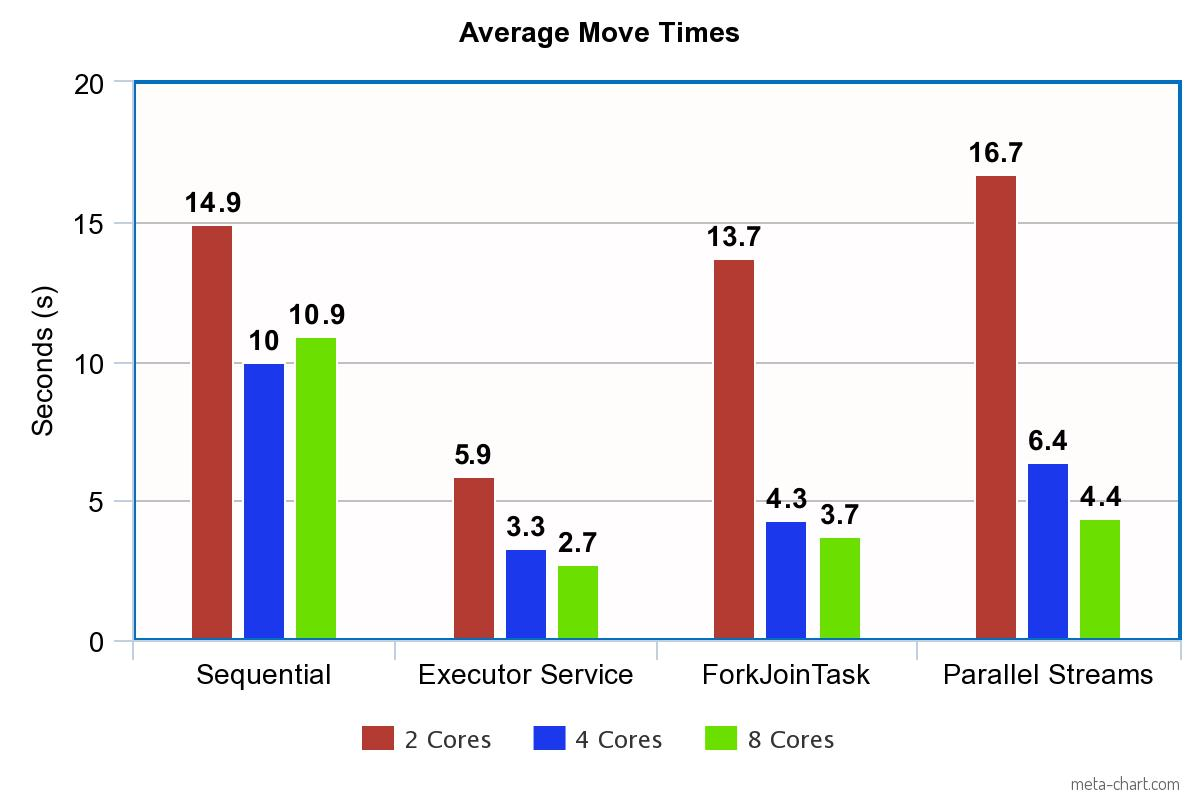
\includegraphics[scale=0.23]{Results-Graph.jpeg}}
\caption{Graph of Results}
\label{fig}
\end{figure}

\section{Evaluation}
\vspace{10pt}

The results from our experiment indicate that Executor Service offers the most optimal performance, followed by Fork/Join and Parallel Streams. The superior performance of Executor Service can be attributed to its ability to maintain a constant thread pool, providing better resource utilization control and minimizing overhead associated with thread creation and management. This constant thread pool, created using ThreadPoolExecutor, ensures that threads are not repeatedly created and destroyed, reducing overhead and aligning well with the iterative control flow of the Alpha-Beta algorithm, making it an effective parallelization method for Alpha-Beta.

ForkJoinTask also performed better than the Sequential, but was not as effective as ExecutorService. Some of the limitations of ForkJoinTasks that may have led to this are:

\begin{itemize}
\item If tasks being executed have varying execution times, the work-stealing algorithm may not effectively balance the workload.
\item Some moves are much more computationally expensive than others, and threads may steal in a suboptimal way, causing some threads to perform much more work than others. This imbalance can lead to decreased performance.
\item Work stealing can lead to cache misses which occur when a worker accesses a subtask that is not in its local cache, causing delays and traffic.
\item Moving work from one thread to another creates overhead that may be computationally expensive.
\end{itemize}

The parallel streams performed the worst of the three parallelized approaches, but still performed better than the Sequential approach. Because Parallel Streams uses the Fork/Join Framework in the background to execute tasks, it also suffers from the same limitations. In addition to these:

\begin{itemize}
\item Functional programming relies heavily on function calls and may produce more intermediate objects than other approaches. This can lead to increased overhead due to function call management and garbage collection, potentially affecting performance.
\end{itemize} \\

\\ Upon examining our findings, it became apparent that Fork/Join and Parallel Streams exhibited a proportionally superior performance on the 8-Core system and 4-Core System compared to the 2-core processor. When comparing this to the sequential results, we see that around 2 cores, these three methods have similar results, but when increasing cores, the sequential results do not improve very much, while the parallel ones improve drastically. This is evidence of the effect that allowing more threads to work increases the performance of the Alpha-Beta algorithm.

In summary, ExecutorService stands out as the most effective parallelism technique in our study for the Alpha-Beta algorithm, but each implementation was able to improve upon the Sequential Algorithm.

\section{Limitations of Research}
\vspace{10pt}

One limitation of the research is the inability to perform testing in a perfectly controlled environment. When performing testing, other programs running on the computer at the time of testing could introduce inaccuracies in the recorded times. We attempted to account for this by averaging the results of 5 games for each method, to reduce the effect error had on the data. \\
Another limitation is the inherent randomness of each game and the varying computation times for each position. This can also introduce inaccuracies, as some positions are quicker to search through the possibilities due to less possible moves. We chose to concentrate on the game's initial 50 moves, which are usually the most computationally demanding, to minimize the impact of randomness.\\
It is important to note that the order the sequential method explores each node will remain consistent, so if the same moves are given to it, it will produce the same result every time. This is not true for the parallel implementations because multiple threads are evaluating nodes simultaneously and the order may be different each time, causing different pruning decisions and alternative moves being selected. This does not necessarily cause move quality to decrease, but would require further testing to evaluate further.


\section{Challenges Encountered}
\vspace{10pt}

Our original parallel implementation, before moving to the context of a chess game, ran substantially slower than the sequential version. This unfortunately held true for every size of tree that we have tested. Trees with larger depths, such as 25, encountered heap size errors when trying to create the tree. When switching to the chess game move trees, we started to actually see improvement.A possible explanation for this is that the sequential algorithm was able to perform much better on a simple tree containing only integer values, that was not as computationally demanding as the context of a chess game, where moves are sent to an evaluator to determine a score for each move. However, more research would be required to determine the true reason. \\
 \\ In our final experiment, we chose to keep the depth constant for this experiment, due to the exponential nature of  hess move trees, when the depth is increased it starts to run extremely slowly and makes it impractical to gather data.


\section{Future Research}
\vspace{10pt}

For future research, it would be worthwhile to evaluate these parallelism techniques on a variety of algorithms beyond the Alpha-Beta to gain a broader understanding of their effectiveness and applicability across various problem areas. This could offer important insights into each method's advantages and drawbacks, assisting in the selection of the most appropriate parallelism technique for distinct computational tasks. Another avenue to explore would be having each implementation play against each other, to gain an idea of where they rank skill-wise.

\section{Conclusion}
\vspace{10pt}

The parallel implementations proved to improve the performance of the Sequential Alpha-Beta Pruning Algorithm for Chess. Due to the large variation in chess games, a larger-scale study could provide more insightful results. We plan to upload a final version of our AI to the Lichess website for anyone to play against.

Our code: \url{https://github.com/cirillojon/ChessAI}

Link to Existing Open-Source Chess AI used: \url{https://github.com/amir650/BlackWidow-Chess}

Research paper regarding parallelizing alpha-beta: \url{https://arxiv.org/pdf/1908.11660.pdf}



\begin{thebibliography}{00}
\bibitem{b1} G. Joanna, How IBM’s Deep Blue Beat World Champion Chess Player Garry Kasparov,'' IEEE Spectrum, 03-May-2017. [Online]. Available: \url{https://spectrum.ieee.org/how-ibms-deep-blue-beat-world-champion-chess-player-garry-kasparov}. [Accessed: 02-Apr-2023]. \bibitem{b2} How Many Possible Moves Are There In Chess?'' Chess Journal, [Online]. Available: \url{https://www.chessjournal.com/how-many-possible-moves-are-there-in-chess/}. [Accessed: 02-Apr-2023].
\bibitem{b3} C. Chang, Java ExecutorService Explained,'' Medium, 08-Jan-2019. [Online]. Available: \url{https://medium.com/@charleschang/java-executorservice-explained-9346b17ce8b4}. [Accessed: 02-Apr-2023]. \bibitem{b4} J. Holbrook, Java Parallel Streams Performance Benchmark,'' Oracle, 25-Aug-2020. [Online]. Available: \url{https://blogs.oracle.com/javamagazine/post/java-parallel-streams-performance-benchmark}. [Accessed: 02-Apr-2023].
\bibitem{b5} ``Fork/Join Framework,'' Oracle, [Online]. Available: \url{https://docs.oracle.com/javase/tutorial/essential/concurrency/forkjoin.html}. [Accessed: 02-Apr-2023].
\end{thebibliography}
\vspace{12pt}


\end{document}